\documentclass{article}

% Math operations
\usepackage{amsmath}

% Insert images from file path
\usepackage{graphicx}
\usepackage{wrapfig}

\usepackage{caption}

% Mono spaced font
\usepackage{bera}

% Referencing figures, listings etc. 
\usepackage{hyperref}
\usepackage{capt-of}

% some color definitions
\usepackage{xcolor}
\definecolor{cblue}{RGB}{16,78,139}
\definecolor{cred}{RGB}{139,37,0}
\definecolor{cgreen}{RGB}{0,139,0} 
\definecolor{corange}{RGB}{255,160,77}
\definecolor{clightblue}{RGB}{62,137,190}

% normal box
\newcommand{\sqboxs}{1.2ex}% the square size
\newcommand{\sqboxf}{0.6pt}% the border in \sqboxEmpty
\newcommand{\sqbox}[1]{\textcolor{#1}{\rule{\sqboxs}{\sqboxs}}}

% Code highlighting
\usepackage{color}
\usepackage{listings}
\usepackage{setspace}

% Define colors for Python listings
\definecolor{Code}{rgb}{0,0,0}
\definecolor{Decorators}{rgb}{0.5,0.5,0.5}
\definecolor{Numbers}{rgb}{0.5,0,0}
\definecolor{MatchingBrackets}{rgb}{0.25,0.5,0.5}
\definecolor{Keywords}{rgb}{0,0,1}
\definecolor{self}{rgb}{0,0,0}
\definecolor{Strings}{rgb}{0,0.63,0}
\definecolor{Comments}{rgb}{0,0.63,1}
\definecolor{Backquotes}{rgb}{0,0,0}
\definecolor{Classname}{rgb}{0,0,0}
\definecolor{FunctionName}{rgb}{0,0,0}
\definecolor{Operators}{rgb}{0,0,0}
\definecolor{Background}{rgb}{0.98,0.98,0.98}

\lstdefinelanguage{Python}{
	numbers=left,
	numberstyle=\footnotesize,
	numbersep=1em,
	xleftmargin=1em,
	framextopmargin=2em,
	framexbottommargin=2em,
	showspaces=false,
	showtabs=false,
	showstringspaces=false,
	frame=l,
	tabsize=4,
	% Basic
	basicstyle=\ttfamily\small\setstretch{1},
	backgroundcolor=\color{Background},
	% Comments
	commentstyle=\color{Comments}\slshape,
	% Strings
	stringstyle=\color{Strings},
	morecomment=[s][\color{Strings}]{"""}{"""},
	morecomment=[s][\color{Strings}]{'''}{'''},
	% keywords
	morekeywords={import,from,class,def,for,while,if,is,in,elif,else,not,and,or,print,break,continue,return,True,False,None,access,as,,del,except,exec,finally,global,import,lambda,pass,print,raise,try,assert},
	keywordstyle={\color{Keywords}\bfseries},
	% additional keywords
	morekeywords={[2]@invariant,pylab,numpy,np,scipy},
	keywordstyle={[2]\color{Decorators}\slshape},
	emph={self},
	emphstyle={\color{self}\slshape},
	%
}
\linespread{1.3}


% Define new float types so that I can reference them with captionof from the capt-of package. 
% https://tex.stackexchange.com/questions/6157/floating-an-algorithm
% Could be helpful as well: https://tex.stackexchange.com/questions/115499/image-caption-within-newfloat
\usepackage{float}
\newfloat{MyListing}{t}{lop}
\newfloat{Enumerate}{t}{lop2}


\begin{document}
	\title{Assignment 1 - Programming Project: Ridge Regression and Model Selection}
	\maketitle
	
	\section{Teammembers and Contributions}
	\begin{itemize}
		\item \makebox[0.55\linewidth]{\textbf{Bernd Menia, \hfill01316129:}} Report, Part Programming
		\item \makebox[0.55\linewidth]{\textbf{Maximilian Samsinger, \hfill01115383:}} Main Programming
	\end{itemize}
	The difference in our contributions is because Bernd just only started working with Machine Learning while Maximilian has already prior knowledge in the subject. Thus we worked together, but the main programming work for this assignment was done by Maximilian.\\
	\\
	Due to the size of the code we will only list the important parts and explain them in detail with the results. 
	
	\section{Prerequisites and Partitioning} 
	\textit{Exercise 1: Choose a nonlinear function $\mathbf{f(x)}$ of a scalar variable $\mathbf{x}$. Generate a data set of $\mathbf{N}$ data points $\mathbf{t_n = f(x_n) + \epsilon}$, where is drawn from a normal distribution with variance.}\\
	\\
	Our data points are denoted by $N$ which we set to 30. There was no mathematical reason for this, but by testing our code with multiple values for $N$ we found 30 to be a fitting number for this assignment. The nonlinear function $f(x) = \sin(2*\pi*x)$ can be seen in \autoref{plot:sine5}. We chose a sine function because it is simplistic and let's us demonstrate the linear regression easily. The blue curve corresponds to the 
	%It demonstrates the ratio between the data- and test points well and also shows the 
	
	%\begin{figure}[h]
	%	\lstinputlisting[language=Python]{code/f.py}
	%	\caption{Test}
	%	\label{code:f}
	%\end{figure}
	
	% https://tex.stackexchange.com/questions/94016/how-to-reduce-space-between-image-and-its-caption
	%\captionsetup[figure]{skip=0pt}
	\begin{wrapfigure}{r}{0.5\textwidth} %this figure will be at the right
		\centering
		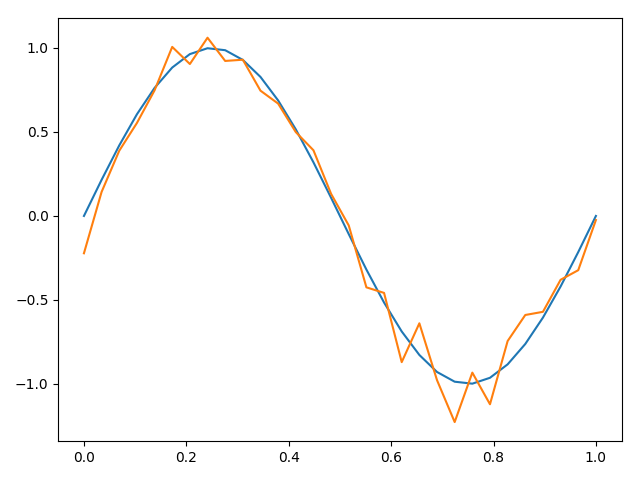
\includegraphics[width=0.5\textwidth]{plots/sine5.png}
		\caption{Initial sine function}
		\sqbox{clightblue} Only $\sin(2*\pi*x)$\\
		\sqbox{corange} Including randomized errors
		\label{plot:sine5}
	\end{wrapfigure}
	%\captionsetup[figure]{skip=10pt}
	
	
	%TODO What happens with the k-fold cross-validation when not all buckets have the same amount of elements? 
	
	The next step is to divide our data points into training- and test sets. We chose to use $\frac{1}{5}$ of all data points rounded down. There is no rule how the points have to be distributed. This also means that we can theoretically distribute the points like we want. Let's assume we have a vector $x$ that holds all x-values for the data- and test points. We could take the first $k = \frac{1}{5}$ elements of the vector for the trainings set and the rest for the test set. However this would most likely be very bad because if the elements are ordered we have a biased test set. Taking the first 2 elements of $[0,1,2,3,4,5,6,7,8,9]$ would give $[0,1]$ which is heavily biased towards lower x-values, or rather the left side of the function. In that case the probability is high that the error function produces a high result.\\
	\\
	A simple solution would be to order the vector and then take re-do the explained procedure. However even by doing this there still is the possibility that the points are not evenly distributed and biased. Randomizing $x$ could still produce the result $[0,1,5,3,7,8,4,9,2,6]$ in which case the trainings points would again be [0,1]. \\
	\\
	There is another solution that fixes this problem without much trouble. First we have to order our vector $x$ and then partition it into $n$ buckets. For example if $n = 2$ then we would split $x$ into 2 as equally big parts as possible. For $x$ this would result in $[[0,1,2,3,4],[5,6,7,8,9]]$. We chose $n$ to be $k = \frac{1}{5}$ of our data points. The second step is to randomize each bucket. This could for example result in $[[3,2,4,1,0],[6,9,8,5,7]]$. Finally we can take 1 element out of each bucket as our test points and the rest as our trainings points. Doing this we can guarantee that there is no bias towards any part of the curve because the buckets are evenly distributed over the x-values.
	
	\section{K-Fold Cross-Validation}
	Doing this is also convenient because we can use the buckets for our K-Fold Cross-Validation. Since our buckets have $k$ elements we iterate $k$ times over all buckets. In each iteration we take the $k-th$ element of each bucket and put them into a new bucket $b$. This new bucket then serves as one fold. $k$ of all elements in the fold are then put into the test set (should always be 1 due to how the buckets got created) and the rest are training points. \\
	
	\section{Calculate the Results}
	With that in mind it is now time to calculate the actual results. To dampen the effect of high amplitudes, due to possible outliers, we included a regularization factor, $\lambda$, in our calculations. The range of our $\lambda$ values is divided into 300 elements, ranging from -37 up to -1 in equal steps. For each lambda we calculate the training- and test errors, as well as the coefficients of our resulting functions. All resulting values get sorted. From there on we chose 3 specific curves to showcase the effect of \textbf{underfitting}, \textbf{overfitting} and \textbf{optimal fitting}. For the underfitting curve we chose the $\lambda$ value were the error for the training set was the highest. (In graph X this value corresponds to Y. Allthough since we use randomized functions the lambda values may change each run). On the contrary the overfitting curve is represented by the $\lambda$ value that has the lowest training error, but comparatively high test error. Finally the optimal fitting curve is simply the curve with the lowest combined training error and test error. All three curves can be seen in Figure X, together with the actual underlying function, the randomized data points and the initial sine function from which we approximated our results. All of the described curves and values are depicted in \autoref{plot:full4cropped}. 
	
	\begin{figure}[h]
		\centering
		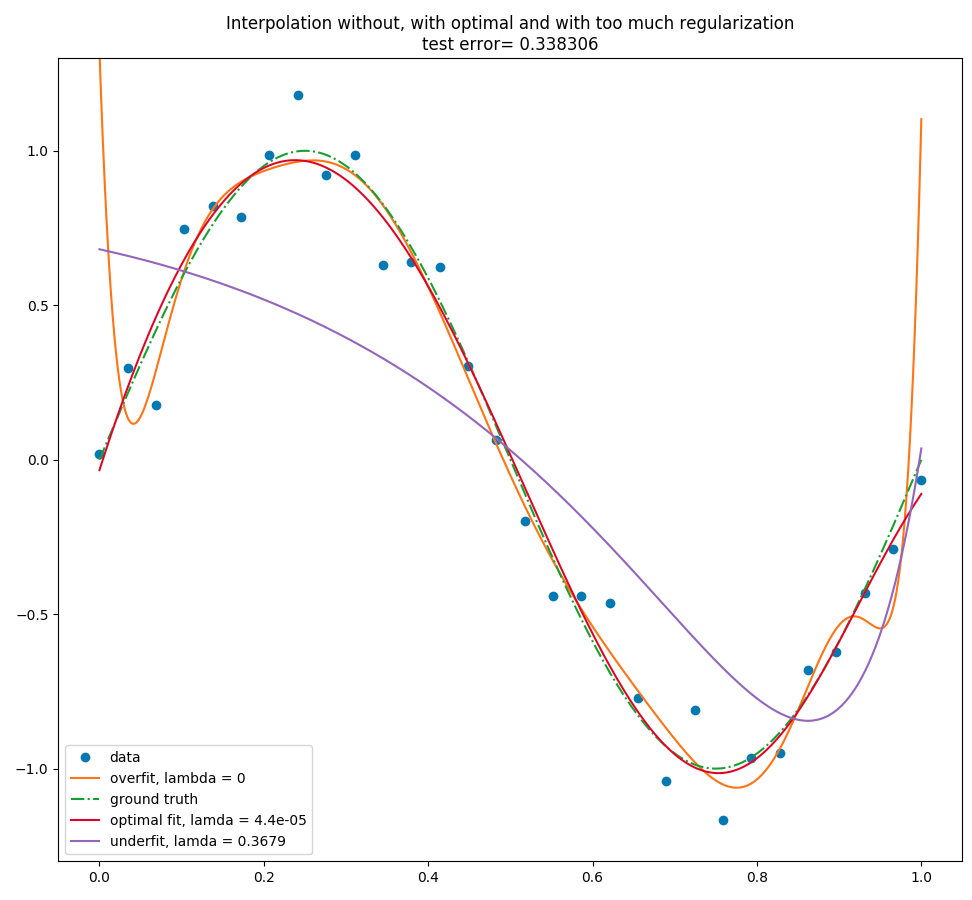
\includegraphics[width=\linewidth]{plots/full4cropped.png}
		\caption{}
		\label{plot:full4cropped}
	\end{figure}
	
	\begin{wrapfigure}{r}{0.5\textwidth} %this figure will be at the right
		\centering
		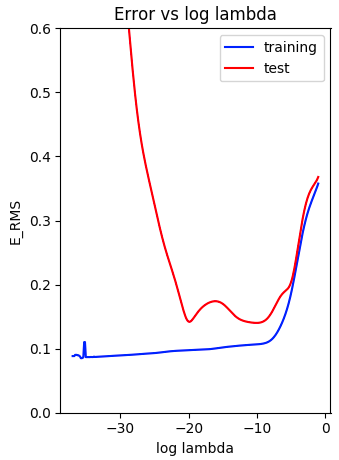
\includegraphics[width=0.5\textwidth]{plots/error4cropped.png}
		\caption{Ratio between the test- and training errors}
		\label{plot:error4cropped}
	\end{wrapfigure}
	
	The ratio between the test- and training errors can be seen in \autoref{plot:error4cropped}. Note that we have taken the natural logarithm of the $\lambda$'s so that we can properly display all values in a small plot. As we can see the more we go to the left of our graph, i.e. the $\lambda$ values get smaller, the overfitting gets increased drastically. The error for the training set stays stays almost the same from about $-8$ to $-37$, however from $-20$ downwards the test errors skyrocket. This represents overfitting of our initial function and can also be seen as the orange curve in \autoref{plot:full4cropped}. The bump between $-20$ and $-10$ is interesting, but (I don't know why this exists). \\
	\\
	\autoref{plot:error4cropped} also shows us underfitting on the right side of the plot. From about $-8$ up to $0$ we can again see that the test errors skyrocket. However in contrast to overfitting, due to the nature of underfitting curves, the training errors also increase. This happens because we try to fit a lower order function to a higher order one of which it simply cannot follow the ups and downs. 
	
	
	
	%\begin{figure}[h]
	%	\centering
	%	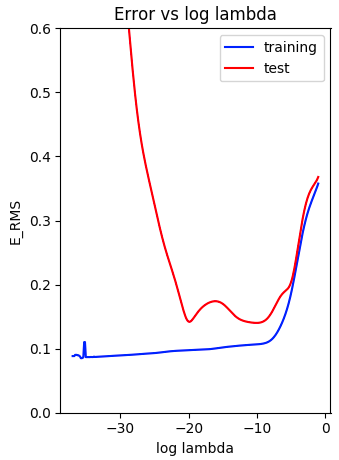
\includegraphics[width=\linewidth]{plots/error4cropped.png}
	%	\caption{Ratio between the test- and training errors}
	%	\label{plot:error4cropped}
	%\end{figure}
	
	%\begin{figure}
	%	\centering	
	%	\captionof{Enumerate}{
	%		What I used the YouTube Data APIv3 for
	%	}
	%	\label{asdf}
	%	
	%	\lstset{
	%		language={Python}
	%	}
	%	\lstinputlisting{code/f.py}
	%\end{figure}
		
		
	
\end{document}